% !TeX root = ../main.tex

\section{การทดลองที่ 1: วัดค่า Spring Constant (\texorpdfstring{$K$}{K})}
\textit{ครอบคลุม Criteria: Part 1 System Modeling --- ออกแบบการทดลองหา $K$, รายงานค่าทางสถิติ (รวม 2 คะแนน)}

%% ─────────────────────────────────────────
\subsection{บทนำ}

ในการสร้างแบบจำลองทางคณิตศาสตร์ของระบบ Mass-Spring-Damper นั้น ค่า Spring Constant หรือ $K$ คือพารามิเตอร์พื้นฐานตัวแรกที่จำเป็นต้องทราบ โดย $K$ คือค่าที่บอกว่าสปริงต้านทานแรงได้มากน้อยเพียงใดต่อหนึ่งหน่วยของการกระจัด ซึ่งอธิบายได้ด้วย Hooke's Law ในรูป $F = Kx$ ค่านี้จะถูกนำไปใช้โดยตรงในการสร้าง State-Space Model และ Equation of Motion ของระบบในการทดลองที่ 4 และ 5 ดังนั้นความแม่นยำของ $K$ จึงส่งผลโดยตรงต่อความถูกต้องของ Kalman Filter ที่จะสร้างขึ้นในภายหลัง

การหาค่า $K$ ทำได้โดยอาศัยหลักการของ Hooke's Law ซึ่งระบุว่าในช่วง Linear Elastic ของสปริง แรงที่กระทำต่อสปริง $F$ จะแปรผันตรงกับระยะที่สปริงยืดหรือหดออกจากตำแหน่งปกติ $x$ โดย $K$ คือความชันของความสัมพันธ์นี้ ในทางปฏิบัติการทดลองนี้จะทำโดยการใส่มวลที่รู้ค่าลงบนสปริงทีละขั้น แล้ววัดระยะกระจัดที่เกิดขึ้นในแต่ละน้ำหนัก จากนั้นนำข้อมูลที่ได้มา Plot กราฟ Force vs.\ Displacement และใช้ Linear Regression หาค่า $K$ จาก Slope ของเส้นตรงที่ได้

อย่างไรก็ตาม ในการรายงานค่า $K$ อย่างน่าเชื่อถือนั้น การวัดเพียงครั้งเดียวไม่เพียงพอ เนื่องจากการทดลองในโลกความเป็นจริงย่อมมีความคลาดเคลื่อนเกิดขึ้นเสมอ ไม่ว่าจะมาจากความไม่สม่ำเสมอของสปริงเอง การอ่านค่าของผู้ทดลอง หรือสปริงที่อาจไม่ได้ตั้งตรงแนวดิ่งอย่างสมบูรณ์ ดังนั้นการทดลองนี้จึงกำหนดให้ทำซ้ำหลายครั้งและใช้วิธีการทางสถิติที่เหมาะสม เช่น ค่าเฉลี่ย ส่วนเบี่ยงเบนมาตรฐาน และค่า $R^2$ ในการประเมินความน่าเชื่อถือของผลลัพธ์ที่ได้

%% ─────────────────────────────────────────
\subsection{วัตถุประสงค์}
\begin{itemize}
    \item เพื่อหาค่า Spring Constant $K$ ของสปริงที่ใช้ในชุดทดลอง Mass-Spring-Damper
    \item เพื่อเลือกและใช้วิธีทางสถิติที่เหมาะสมในการรายงานค่า $K$ อย่างน่าเชื่อถือ
    \item เพื่อยืนยันว่าสปริงทำงานในช่วง Linear Elastic ตาม Hooke's Law
\end{itemize}

%% ─────────────────────────────────────────
\subsection{สมมติฐาน}
\begin{itemize}
    \item ความสัมพันธ์ระหว่างแรงและการกระจัดของสปริงจะเป็นเชิงเส้น (Linear) ในช่วงน้ำหนักที่ทดสอบ
    \item ค่า $K$ ที่ได้จาก Linear Regression จะมีความสม่ำเสมอและค่า $R^2$ สูง
\end{itemize}

%% ─────────────────────────────────────────
\subsection{ตัวแปร}
\begin{enumerate}
    \item \textbf{ตัวแปรต้น (Independent Variable):} มวลที่กระทำต่อสปริง โดยทำการเพิ่มน็อตตัวเมียทีละ 1 ตัว น้ำหนักประมาณตัวละ 38 g (เพิ่มได้สูงสุด 5 ตัว รวมน้ำหนักสูงสุด 190 g)
    \item \textbf{ตัวแปรตาม (Dependent Variable):} ระยะการกระจัด $x$ (m) ที่เกิดขึ้นในแต่ละระดับน้ำหนัก
    \item \textbf{ตัวแปรควบคุม (Control Variables):}
    \begin{itemize}
        \item ชนิดและค่าความแข็งเดิมของสปริงที่ใช้ทดสอบ
        \item อุณหภูมิห้องและสภาพแวดล้อม
        \item ทิศทางการแขวนสปริง (ต้องอยู่ในแนวดิ่งเสมอเพื่อป้องกันแรงเสียดทานด้านข้าง)
        \item ตำแหน่ง Reference เริ่มต้นก่อนทำการโหลดมวล
    \end{itemize}
\end{enumerate}

%% ─────────────────────────────────────────
\subsection{เอกสารและงานวิจัยที่เกี่ยวข้อง}

\subsubsection{กฎของฮุก (Hooke's Law) และข้อสมมติของวัสดุยืดหยุ่นเชิงเส้น}

\paragraph{ความหมายและความสำคัญของกฎของฮุก}

กฎของฮุกเป็นทฤษฎีพื้นฐานทางกลศาสตร์วัสดุที่ใช้อธิบายความสัมพันธ์ระหว่างแรงที่กระทำต่อวัสดุกับการเปลี่ยนรูปที่เกิดขึ้น โดย Robert Hooke ได้เสนอหลักการนี้ในปี ค.ศ.\ 1678 ซึ่งระบุว่า:
\begin{itemize}
    \item ภายในช่วงยืดหยุ่นของวัสดุ (Elastic Region) การเปลี่ยนรูปของวัสดุจะแปรผันตรงกับแรงที่กระทำ
    \item เมื่อแรงที่กระทำเพิ่มขึ้น การยืดตัวหรือการเสียรูปของวัสดุจะเพิ่มขึ้นตามสัดส่วนเดียวกัน
    \item ตราบใดที่วัสดุยังไม่เกินขีดจำกัดการยืดหยุ่น (Elastic Limit) ความสัมพันธ์นี้ยังคงมีผลบังคับใช้
\end{itemize}

\paragraph{ความสัมพันธ์ระหว่างความเค้นและความเครียด}

ความสัมพันธ์ดังกล่าวสามารถอธิบายได้ผ่านสมการทางคณิตศาสตร์ดังนี้
\begin{equation}
    \sigma = E \varepsilon
\end{equation}
โดยที่:
\begin{itemize}
    \item $\sigma$ คือความเค้น (Stress) แรงที่กระทำต่อพื้นที่หนึ่งหน่วย
    \item $\varepsilon$ คือความเครียด (Strain) การเปลี่ยนแปลงรูปร่างสัมพัทธ์ของวัสดุ
    \item $E$ คือมอดูลัสยัง (Young's Modulus) ตัวบ่งบอกความแข็งของวัสดุ
\end{itemize}

หากวัสดุมีค่า Young's Modulus สูง จะสามารถต้านทานการเปลี่ยนรูปได้มากกว่าวัสดุที่มีค่า Young's Modulus ต่ำ

\paragraph{การประยุกต์ใช้กฎของฮุกกับระบบสปริง}

สำหรับระบบสปริง กฎของฮุกสามารถอธิบายในรูปความสัมพันธ์ระหว่างแรงกับการกระจัด ดังสมการต่อไปนี้
\begin{equation}
    F = K x
    \label{eq:hooke}
\end{equation}
โดยที่:
\begin{itemize}
    \item $F$ คือแรงที่กระทำ (หน่วย: นิวตัน)
    \item $K$ คือค่าคงที่ของสปริง (Spring Constant) ตัวแสดงความแข็งของสปริง
    \item $x$ คือระยะยืดตัว (Displacement)
\end{itemize}

สมการนี้แสดงให้เห็นว่า:
\begin{itemize}
    \item การยืดตัวของสปริงมีความสัมพันธ์เชิงเส้นกับแรงที่กระทำ
    \item ค่าความชันของกราฟแรง-การกระจัดสามารถใช้แทนค่าคงที่ของสปริงได้
\end{itemize}

\begin{figure}[htbp]
    \centering
    
\includegraphics[width=0.6\textwidth]{exp1_hookes_law.jpg}
    \caption{แผนภาพแสดงกฎของฮุก (Hooke's Law)}
    \label{fig:hookes_law}
\end{figure}

\subsubsection{ข้อสมมติของวัสดุยืดหยุ่นเชิงเส้น (Linear Elastic Assumptions)}

\begin{itemize}
    \item \textbf{ข้อสมมติที่ 1 ความสัมพันธ์เชิงเส้นระหว่างความเค้นและความเครียด:} วัสดุต้องมีความสัมพันธ์ระหว่างความเค้นและความเครียดเป็นเชิงเส้น และต้องเป็นไปตามกฎของฮุกอย่างสมบูรณ์ภายในช่วง Elastic Region เท่านั้น
    \item \textbf{ข้อสมมติที่ 2 สมมติการเปลี่ยนรูปเล็กน้อย (Small Deformation Assumption):} การเปลี่ยนรูปของวัสดุต้องมีขนาดเล็กจนสามารถละเลยผลของการเปลี่ยนแปลงทางเรขาคณิตได้
    \item \textbf{ข้อสมมติที่ 3 ความสามารถในการคืนรูป (Reversibility):} วัสดุต้องสามารถคืนรูปได้เมื่อยกเลิกแรงกระทำ ไม่เกิดการเสียรูปถาวร
    \item \textbf{ข้อสมมติที่ 4 สมบัติเชิงกลคงที่:} สมบัติเชิงกลของวัสดุ เช่น Young's Modulus และ Poisson's Ratio ต้องคงที่ตลอดช่วงการรับแรง
    \item \textbf{ข้อสมมติที่ 5 หลักการซ้อนทับ (Superposition Principle):} ผลตอบสนองรวมของระบบที่เกิดจากแรงหลายแรงสามารถหาได้จากผลรวมของผลตอบสนองที่เกิดจากแต่ละแรงแยกกัน
\end{itemize}

\subsubsection{วิธีการทางสถิติ (Statistical Methods)}

\paragraph{ค่าเฉลี่ย (Mean)}

ค่าเฉลี่ยเป็นตัวชี้วัดแนวโน้มเข้าสู่ส่วนกลางของข้อมูล ใช้แสดงค่าตัวแทนของชุดข้อมูลจากการวัดซ้ำ โดยคำนวณจากสมการ
\begin{equation}
    \bar{x} = \frac{1}{N}\sum_{i=1}^{N} x_i
    \label{eq:mean}
\end{equation}
โดยที่ $\bar{x}$ คือค่าเฉลี่ย, $x_i$ คือค่าข้อมูลแต่ละตัว, และ $N$ คือจำนวนข้อมูลทั้งหมด

\paragraph{ส่วนเบี่ยงเบนมาตรฐาน (Standard Deviation)}

ส่วนเบี่ยงเบนมาตรฐานเป็นเครื่องมือที่ใช้วัดการกระจายตัวของข้อมูลจากค่าเฉลี่ย โดยคำนวณได้จากสมการ
\begin{equation}
    s = \sqrt{\frac{\sum_{i=1}^{N}(x_i - \bar{x})^2}{N-1}}
    \label{eq:std}
\end{equation}

\paragraph{สัมประสิทธิ์ความแปรปรวน (Coefficient of Variation: CV)}

สัมประสิทธิ์ความแปรปรวนเป็นอัตราส่วนระหว่างส่วนเบี่ยงเบนมาตรฐานกับค่าเฉลี่ย และแสดงในรูปเปอร์เซ็นต์
\begin{equation}
    CV = \frac{s}{\bar{x}} \times 100\%
    \label{eq:cv}
\end{equation}

\subsubsection{การวิเคราะห์การถดถอยเชิงเส้น (Linear Regression)}

การวิเคราะห์การถดถอยเชิงเส้นเป็นเครื่องมือสำคัญในการศึกษาความสัมพันธ์ระหว่างตัวแปร สมการพื้นฐานของการถดถอยเชิงเส้นสามารถเขียนได้เป็น
\begin{equation}
    y = mx + c
\end{equation}
โดยที่ $y$ คือตัวแปรตาม, $x$ คือตัวแปรอิสระ, $m$ คือความชัน (Slope), และ $c$ คือจุดตัดแกน (Intercept)

สำหรับการทดลองที่เกี่ยวข้องกับกฎของฮุก เมื่อบังคับให้เส้นตรงผ่านจุดกำเนิด (Intercept = 0) สูตร Slope จาก Regression ผ่านจุดกำเนิดคือ
\begin{equation}
    K = \frac{\displaystyle\sum_{i=1}^{n} F_i \cdot \Delta x_i}{\displaystyle\sum_{i=1}^{n} (\Delta x_i)^2}
    \label{eq:regression_slope}
\end{equation}

\paragraph{สัมประสิทธิ์การตัดสินใจ ($R^2$)}

ค่า $R^2$ ใช้วัดระดับความสอดคล้องของข้อมูลกับเส้นแนวโน้ม หากค่า $R^2$ มีค่าเข้าใกล้ 1 (เช่น 0.95 ขึ้นไป) แสดงว่าข้อมูลมีความสัมพันธ์เชิงเส้นที่ดีและสอดคล้องกับแบบจำลองทางทฤษฎี

%% ─────────────────────────────────────────
\subsection{ขั้นตอนการทดลอง}

\begin{enumerate}
    \item ติดตั้งสปริงในแนวดิ่งกับชุดทดลอง จากนั้นกำหนดตำแหน่ง Reference โดยวัดระยะจากปลายสปริงถึงจุดอ้างอิงขณะยังไม่มีโหลดใดๆ บันทึกเป็น $x_\text{ref}$
    \item ใส่น็อตตัวเมียทีละหนึ่งตัวจนครบ 5 ตัว เพราะน้ำหนักสูงสุดที่ใส่ได้คือ น็อต 5 ตัว โดยชั่งมวลน็อตแต่ละชุดสะสมก่อนทดลองเพื่อให้ทราบค่า $m$ ที่แน่นอน แล้วคำนวณแรงกระทำที่แต่ละระดับโหลดด้วย
    \begin{equation}
        F = mg, \quad g = 9.81 \; \text{m/s}^2
        \label{eq:weight}
    \end{equation}
    \item วัดระยะ $x$ จากตำแหน่ง Reference ที่แต่ละระดับโหลด ทำซ้ำ 3 ครั้งต่อระดับโดยถอดและใส่โหลดใหม่ทุกครั้ง เพื่อหาค่าเฉลี่ยและลด Bias จากการอ่านค่าซ้ำในตำแหน่งเดิม บันทึกเป็น $x_1$, $x_2$, $x_3$ และคำนวณการกระจัดสุทธิ
    \begin{equation}
        \Delta x = \bar{x} - x_\text{ref}
        \label{eq:displacement}
    \end{equation}
    \item Plot กราฟ $F$ (แกน $y$) เทียบกับ $\Delta x$ (แกน $x$) และ Fit เส้นตรงผ่านจุดกำเนิด (Intercept = 0) ด้วย Linear Regression เพื่อให้สอดคล้องกับ Hooke's Law: $F = K \cdot \Delta x$
    \item อ่านค่า $K$ จาก Slope ของ Regression Line คำนวณ Mean และ Standard Deviation ของ $K_i$ จาก Point Estimate แต่ละจุด รวมถึงค่า $R^2$ เพื่อยืนยันความเป็นเชิงเส้น
    \begin{equation}
        K_i = \frac{F_i}{\Delta x_i}, \qquad
        \bar{K} = \frac{1}{n}\sum_{i=1}^{n} K_i, \qquad
        S.D.(K) = \sqrt{\frac{\sum(K_i - \bar{K})^2}{n-1}}
        \label{eq:k_stats}
    \end{equation}
    การเลือกใช้ 5 ระดับโหลด (6 จุดข้อมูลรวมจุดกำเนิด) เป็นจำนวนขั้นต่ำที่ทำให้ Linear Regression
มีระดับความเป็นอิสระ (Degree of Freedom) เพียงพอสำหรับการประมาณค่า $K$ และ Intercept 
พร้อมกันโดยไม่เกิด Overfitting อย่างไรก็ตาม หากเพิ่มจำนวนจุดข้อมูลมากขึ้น ค่า Slope ที่ได้จะมี 
Standard Error ลดลง ทำให้ค่า $K$ มีความน่าเชื่อถือสูงขึ้น แต่ต้องแลกกับเวลาและความพยายามในการ
ทดลองที่เพิ่มขึ้นด้วย
\end{enumerate}

% \begin{figure}[htbp]
%     \centering
%     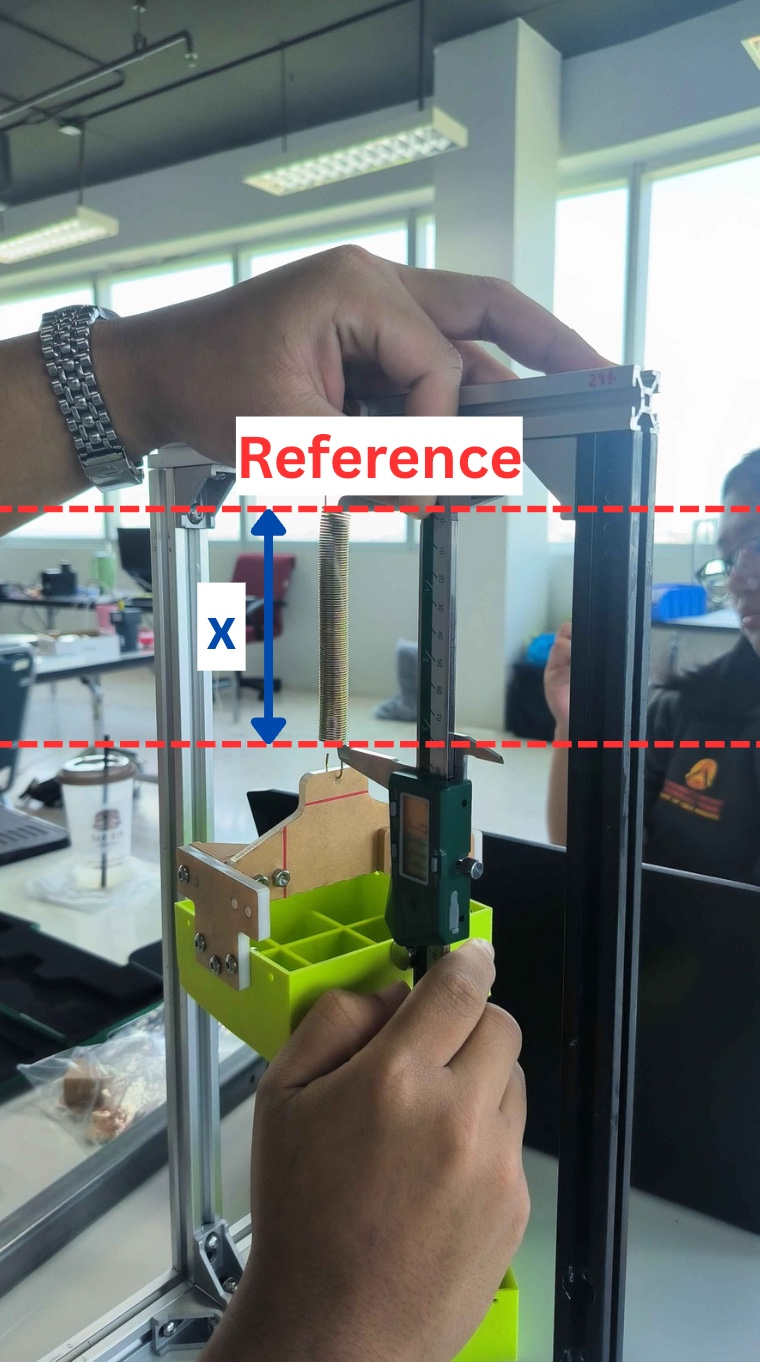
\includegraphics[width=0.35\textwidth]{images/SCR-20260420-octm.jpeg}
%     \caption{ชุดทดลองที่ติดตั้งสปริงในแนวดิ่ง พร้อม Reference Point และตำแหน่งวัด}
%     \label{fig:exp1_setup}
% \end{figure}

%% ─────────────────────────────────────────
\subsection{ผลการทดลอง}

\subsubsection{ตารางข้อมูลที่บันทึกได้}

ตารางด้านล่างแสดงค่าแรงที่กระทำต่อสปริง ($F = mg$) และค่าการกระจัดเฉลี่ย ($\bar{x}$) พร้อมส่วนเบี่ยงเบนมาตรฐาน (S.D.) ที่ได้จากการวัด 3 ครั้งในแต่ละระดับโหลด โดยกำหนดตำแหน่ง Reference ที่ไม่มีโหลดเป็น $x_\text{ref} = 93.272$ mm และคำนวณการกระจัดสุทธิ $\Delta x = \bar{x} - x_\text{ref}$
% การแสดงผลตารางสรุปค่าเฉลี่ยจากการทดลอง
% อ้างอิงหน่วยตามที่ระบุในข้อมูลชุดล่าสุด
\begin{table}[ht]
    \centering
    \caption{ตารางสรุปผลการทดลองหาค่า Spring Constant (เฉพาะค่าเฉลี่ย)}
    \label{tab:spring_summary}
    \begin{tabular}{ccccc}
        \hline
        \textbf{มวลเฉลี่ย $\bar{m}$ (kg)} & \textbf{แรง $F=mg$ (N)} & \textbf{ระยะเฉลี่ย $\bar{x}$ (m)} & \textbf{S.D. ของ $x$ (mm)} & \textbf{S.D. ของ $m$ (g)} \\
        \hline
        % ข้อมูลชุดที่ 1: ตำแหน่งอ้างอิง (No Load)
        0.000 & 0.000 & 0.094 & 0.045 & 0.000 \\
        % ข้อมูลชุดที่ 2: โหลดระดับที่ 1
        0.038 & 0.372 & 0.106 & 1.133 & 0.115 \\
        % ข้อมูลชุดที่ 3: โหลดระดับที่ 2
        0.076 & 0.743 & 0.118 & 1.234 & 0.153 \\
        % ข้อมูลชุดที่ 4: โหลดระดับที่ 3
        0.114 & 1.116 & 0.131 & 1.437 & 0.379 \\
        % ข้อมูลชุดที่ 5: โหลดระดับที่ 4
        0.152 & 1.488 & 0.144 & 0.866 & 0.208 \\
        % ข้อมูลชุดที่ 6: โหลดระดับที่ 5
        0.190 & 1.860 & 0.158 & 1.281 & 0.289 \\
        \hline
    \end{tabular}
        \begin{minipage}{0.85\textwidth}
        \vspace{4pt}
        \footnotesize
        \textit{หมายเหตุ:} ค่า $\bar{x}$ ในตารางนี้แสดงผลแบบ Round เพื่อความกระชับ
        ค่า $\Delta x$ ที่ใช้คำนวณจริงในตารางที่~\ref{tab:k_pointest}
        คำนวณจากข้อมูลดิบก่อน Round ดังนั้นจึงมีทศนิยมมากกว่า
    \end{minipage}
\end{table}

\begin{figure}[htbp]
    \centering
    
\includegraphics[width=0.75\textwidth]{exp1_force_dist.png}
    \caption{กราฟแสดงผลการทดลองระหว่างแรงกับการกระจัด}
    \label{fig:force_displacement}
\end{figure}

\subsubsection{การคำนวณค่า \texorpdfstring{$K$}{K} ด้วย Linear Regression}

จาก Hooke's Law ความสัมพันธ์ระหว่างแรงและการกระจัดอยู่ในรูป $F = K \cdot \Delta x$
ดังนั้น $K$ คือความชันของเส้นตรง (Slope) ที่ได้จากการทำ Linear Regression
ของข้อมูล Force vs.\ Displacement

ในการวิเคราะห์นี้ใช้สองแนวทาง ได้แก่ \textbf{(1) OLS ผ่านจุดกำเนิด}
ซึ่งตรงกับนิยามของ Hooke's Law โดยตรง และ
\textbf{(2) Full OLS with Intercept} ซึ่งอนุญาตให้มี Offset คงที่
เพื่อรองรับความคลาดเคลื่อนเชิงระบบของการตั้งค่าอุปกรณ์

\paragraph{แนวทางที่ 1: OLS ผ่านจุดกำเนิด}

บังคับให้ Intercept = 0 ตามนิยามของ Hooke's Law ($F = K \cdot \Delta x$)
สูตรที่ใช้คือ
\begin{equation}
    K_{\text{origin}} =
    \frac{\displaystyle\sum_{i=1}^{n} (F_i \cdot \Delta x_i)}
         {\displaystyle\sum_{i=1}^{n} (\Delta x_i)^2}
    = \frac{0.257951}{0.008746}
    \approx 29.49 \; \text{N/m}
\end{equation}

\paragraph{แนวทางที่ 2: Full OLS with Intercept (ค่าที่เลือกใช้)}

เมื่อ Plot กราฟ $F$ vs.\ $\Delta x$ พบว่าเส้น Regression ไม่ผ่านจุดกำเนิดพอดี
แต่มี Offset เล็กน้อย ซึ่งสะท้อนถึง Systematic Error จากการกำหนด Reference
Position ($x_\text{ref}$) ที่มี Measurement Noise เล็กน้อย
จึงใช้ Full OLS ในรูป $F = K \cdot \Delta x + c$ เพื่อจัดการ Offset นี้
\begin{equation}
    \boxed{K = 29.11 \; \text{N/m}} \quad,\quad c = 0.0163 \; \text{N}
\end{equation}
ค่า $K = 29.11$ N/m นี้จะถูกนำไปใช้ในการทดลองที่ 4 และ 5 ทั้งหมด
เนื่องจาก Full OLS ลด Bias จาก Systematic Offset ได้ดีกว่า OLS ผ่านจุดกำเนิด

% --- Section: Spring Constant Analysis ---
\subsection{ผลการวิเคราะห์ค่าคงที่สปริง (Spring Constant Analysis)}

จากการทดลองหาความสัมพันธ์ระหว่างแรง $F$ และระยะยืด $\Delta x$ เพื่อหาค่าคงที่สปริง $K$ ตามกฎของฮุก ($F = k\Delta x$) สามารถสรุปผลการวิเคราะห์เชิงสถิติได้ดังนี้

\subsubsection{การวิเคราะห์ด้วยวิธีการถดถอยเชิงเส้น (Linear Regression)}

จากการวิเคราะห์ใน Section 1.7.2 ด้วย Full OLS ได้ผลลัพธ์:
\begin{equation}
    \boxed{K = 29.11 \; \text{N/m}} \quad,\quad c = 0.0163 \; \text{N}
\end{equation}
เมื่อ $c$ คือ Systematic Offset ของระบบการวัด
ค่า $K = 29.11$ N/m ถูกเลือกเป็นค่าสุดท้ายเนื่องจาก Full OLS
จัดการ Offset ได้ดีกว่า OLS ผ่านจุดกำเนิด (ซึ่งให้ $K_\text{origin} = 29.49$ N/m)

\subsubsection{ค่าทางสถิติและจุดประมาณการ (Point Estimates)}

เพื่อตรวจสอบความสม่ำเสมอของค่าคงที่สปริงในแต่ละช่วงน้ำหนัก จึงคำนวณค่า $K_i$ ณ แต่ละระดับโหลดโดยใช้ความสัมพันธ์ $K_i = F_i / \Delta x_i$ ผลลัพธ์แสดงดังตารางที่ \ref{tab:k_pointest}:

\begin{table}[h]
    \centering
    \caption{ค่า Point Estimate ของ $K$ ที่แต่ละระดับโหลด}
    \label{tab:k_pointest}
    \begin{tabular}{cccc}
        \hline
        \textbf{ระดับโหลด} & \textbf{$F_i$ (N)} & \textbf{$\Delta x_i$ (m)} & \textbf{$K_i$ (N/m)} \\
        \hline
        1 & 0.372 & 0.01222 & 30.44 \\
        2 & 0.743 & 0.02429 & 30.59 \\
        3 & 1.116 & 0.03735 & 29.88 \\
        4 & 1.488 & 0.05007 & 29.72 \\
        5 & 1.860 & 0.06407 & 29.03 \\
        \hline
    \end{tabular}
\end{table}

จากการคำนวณหาค่าเฉลี่ย ($\bar{K}$) และค่าเบี่ยงเบนมาตรฐาน (S.D.) ของกลุ่มตัวอย่าง:
\begin{equation}
    \bar{K} = \frac{\sum_{i=1}^{n} K_i}{n} = 29.93 \; \text{N/m}
\end{equation}
\begin{equation}
    S.D.(K) = \sqrt{\frac{\sum_{i=1}^{n} (K_i - \bar{K})^2}{n-1}} \approx 0.63 \; \text{N/m}
\end{equation}
\textbf{หมายเหตุ:} ค่าเฉลี่ย $29.93$ N/m มีค่าสูงกว่าค่าจากการถดถอยเชิงเส้นเล็กน้อย เนื่องจากการคำนวณรายจุดไม่ได้พิจารณาค่าความคลาดเคลื่อนคงที่ ($c$) ของเครื่องมือวัด

\subsubsection{การคำนวณค่าสัมประสิทธิ์การตัดสินใจ (\texorpdfstring{$R^2$}{R^2})}

เพื่อประเมินความแม่นยำของโมเดล $F = 29.11 \Delta x + 0.0163$ จึงทำการคำนวณค่า $R^2$ สำหรับการถดถอยเชิงเส้น ดังนี้:
\begin{equation}
    R^2 = 1 - \frac{SS_{\text{res}}}{SS_{\text{tot}}} = 1 - \frac{\sum_{i=1}^{n} (F_i - \hat{F}_i)^2}{\sum_{i=1}^{n} (F_i - \bar{F})^2}
\end{equation}
โดยที่ $\hat{F}_i$ คือค่าแรงที่ทำนายจากสมการ และ $\bar{F} = 0.93$ N คือค่าเฉลี่ยของแรงทั้งหมด

\begin{table}[ht]
    \centering
    \caption{ตารางคำนวณ Residuals สำหรับการตรวจสอบค่า $R^2$}
    \label{tab:r2_calc}
    \begin{tabular}{cccccc}
        \hline
        $i$ & $\Delta x_i$ (m) & $F_i$ (N) & $\hat{F}_i$ (N) & $(F_i - \hat{F}_i)^2$ & $(F_i - \bar{F})^2$ \\
        \hline
        1 & 0.00000 & 0.000 & 0.0163 & 0.000266 & 0.8643 \\
        2 & 0.01222 & 0.372 & 0.3721 & 0.000000 & 0.3060 \\
        3 & 0.02429 & 0.743 & 0.7234 & 0.000384 & 0.0347 \\
        4 & 0.03735 & 1.116 & 1.1034 & 0.000159 & 0.0360 \\
        5 & 0.05007 & 1.488 & 1.4740 & 0.000196 & 0.3117 \\
        6 & 0.06407 & 1.860 & 1.8814 & 0.000458 & 0.8655 \\
        \hline
        \textbf{Sum} & & & & \textbf{0.001463} & \textbf{2.4182} \\
        \hline
    \end{tabular}
\end{table}

แทนค่าเพื่อหาผลลัพธ์:
\begin{equation}
    R^2 = 1 - \frac{0.001463}{2.4182} \approx 0.9994
\end{equation}
ค่า $R^2$ ที่เข้าใกล้ 1 ยืนยันว่าสมการเชิงเส้นนี้สามารถอธิบายพฤติกรรมของสปริงได้อย่างครอบคลุม

% --- Section: Discussion and Conclusion ---
\subsection{สรุปและอภิปรายผล}

\begin{itemize}
    \item \textbf{สรุปผล:} เลือกรายงานค่าคงที่สปริง $K = 29.11$ N/m จากวิธี Linear Regression เนื่องจากให้ค่า $R^2 = 0.9994$ ซึ่งแสดงถึงความแม่นยำสูง และสามารถจัดการกับค่า Offset ($c = 0.0163$ N) ของระบบได้ดีกว่าการหาค่าเฉลี่ยรายจุด
    \item \textbf{อภิปรายผล:} ความคลาดเคลื่อน (S.D. $\approx 0.63$ N/m) ส่วนใหญ่เกิดจาก Measurement Noise ในการอ่านค่าระยะยืดด้วยสายตา อย่างไรก็ตาม ค่า $K$ ที่ได้มีความเสถียรเพียงพอสำหรับการนำไปประยุกต์ใช้ใน State-Space Model
    \item \textbf{การนำไปใช้:} ค่า $K = 29.11$ N/m จะถูกนำไปบรรจุลงใน System Matrix ของ Kalman Filter เพื่อใช้ในการพยากรณ์สถานะ (State Prediction) ของระบบมวล-สปริงในการทดลองขั้นต่อไป
\end{itemize}